\documentclass[10pt,twocolumn]{article}
\usepackage[accepted]{icml2026}
\usepackage{xspace}

% Convenience macros
\newcommand{\ie}{i.e.\@\xspace}
\newcommand{\eg}{e.g.\@\xspace}
\newcommand{\cf}{cf.\@\xspace}
\newcommand{\etal}{et~al.\@\xspace}
\newcommand{\gemma}{Gemma~3\xspace}
\newcommand{\gemmascope}{GemmaScope~2\xspace}

\icmltitle{Split Personality: Instruction Tuning Decouples Awareness from Defense Against Attentional Hijacking}
\icmltitlerunning{Split Personality: IT Decouples Awareness from Defense}

\icmlauthor{Vincent Ohprecio}{indep}
\icmlaffiliation{indep}{Independent Researcher}
\icmlcorrespondingauthor{Vincent Ohprecio}{ohprecio@gmail.com}
\icmlkeywords{mechanistic interpretability, multi-agent systems, adversarial robustness, sparse autoencoders, alignment}

\begin{document}
\maketitle

%% ============================================================
%% ABSTRACT
%% ============================================================
\begin{abstract}
Multi-agent LLM systems are vulnerable to a subtle attack: selective framing using exclusively true statements.
We identify this mechanism---\emph{attentional hijacking}---and show that instruction tuning (RLHF) makes it strictly worse by decoupling awareness circuits from defense circuits.
Using sparse autoencoder (SAE) features from \gemmascope across \gemma models at 4B, 12B, and 27B parameters, we demonstrate a \emph{dissociation scaling trend}: awareness--task coupling drops from 30.2\% to 4.6\% recovery as model scale increases.
At 27B, instruction-tuned models show 86.3\% task-feature suppression while still mentioning the suppressed information verbally---a behavioral--representational split we term the \emph{Groot effect}.
Base (pretrained) models retain awareness--defense coupling (49.3\% recovery vs.\ 4.6\%), confirming RLHF as the causal factor; SAE-level replication on Llama~3.1 8B shows the same IT-vs-base pattern ($d = 1.61$ vs.\ $1.10$), demonstrating cross-family generality.
The hijacking mechanism is orthogonal to alignment faking (cosine similarity $-0.048$, top-50 feature overlap $=0$), requiring independent defenses.
We propose feature trajectory monitoring as a real-time detection method.
\end{abstract}

%% ============================================================
%% 1. INTRODUCTION
%% ============================================================
\section{Introduction}
\label{sec:intro}

Large language models (LLMs) are increasingly deployed in multi-agent architectures where several model instances collaborate on complex tasks \citep{du2023improving, hong2023metagpt}.
A growing body of work has examined adversarial attacks against individual models through prompt injection and jailbreaking \citep{zou2023universal, wei2024jailbroken}.
However, a qualitatively different vulnerability emerges in multi-agent settings: one agent can undermine another's reasoning \emph{without any false statements}, using only selective emphasis of true information---what we term \emph{attentional hijacking}.

This is not a theoretical concern.
In over 1,500 experiments across six multi-agent campaigns with 2--8 agents and 0--50\% adversarial ratios, we observe that chaos agents using \emph{only verifiable true statements} suppress exploration of valid solution branches by up to 29.8 percentage points, with a phase boundary at approximately 37.5\% adversarial ratio \citep{oh2026civil}.
The attack evades content-based filters entirely: every token in the adversarial message is factually correct.
The damage arises from how the recipient model \emph{allocates attention} across its context---one cannot build a guardrail against true statements.

More troublingly, we discover that \emph{instruction tuning makes models more vulnerable, not less}.
RLHF and related alignment procedures install awareness of contextual manipulation---models can detect when they are being steered---but this awareness is decoupled from the model's ability to resist the steering.
We formalize this as a \textbf{dissociation scaling trend}: as model scale increases from 4B to 27B parameters, the gap between awareness features and task-defense features widens monotonically, from entangled (30.2\% recovery) to fully independent (4.6\% recovery).

The most striking manifestation of this dissociation is what we call the \textbf{Groot effect}: at 27B parameters, the instruction-tuned model verbally mentions the correct answer branch while its internal task features are 86.3\% suppressed.
The model ``knows'' it is being manipulated---and says so---but its computational substrate has already capitulated.
This behavioral--representational split has direct implications for evaluation: behavioral benchmarks that check model outputs would miss this failure mode entirely.

Our contributions are:
\begin{enumerate}
    \item \textbf{Mechanistic identification.} Using SAE feature decomposition on \gemma 4B, we isolate the hijacking mechanism at the feature level: specific task features are completely suppressed (feature 1716 drops from activation 220 to 0) while awareness features remain active. We validate these features on held-out prompts (85\% replication, $p = 8 \times 10^{-6}$) and across three domains (\S\ref{sec:mechanism}).
    \item \textbf{Dissociation scaling trend.} Scaling to 12B and 27B, we show awareness--defense coupling degrades monotonically with scale (\S\ref{sec:scaling}).
    \item \textbf{Causal evidence from IT vs.\ PT.} Comparing instruction-tuned and pretrained 27B models across three ablation methods, we establish post-training (SFT + RLHF) as the causal factor, with cross-family replication on Llama~3.1 8B (\S\ref{sec:it_creates}).
    \item \textbf{Orthogonality to alignment faking.} We show the hijacking feature subspace is orthogonal to alignment-faking features (cosine similarity $-0.048$, Spearman $\rho = 0.008$), requiring independent defenses (\S\ref{sec:orthogonality}).
    \item \textbf{Defense directions.} We outline feature trajectory monitoring as a candidate detection method and identify the signal properties that would enable it (\S\ref{sec:defense}).
\end{enumerate}

%% ============================================================
%% 2. RELATED WORK
%% ============================================================
\section{Related Work}
\label{sec:related}

\paragraph{Sycophancy and Social Pressure.}
\citet{perez2022discovering} showed that LLMs adjust their outputs based on perceived user preferences, and \citet{sharma2023towards} systematically characterized sycophancy as a failure of robustness to social pressure.
Our work extends this line by identifying a \emph{mechanistic} pathway---attention reallocation---through which social pressure operates, and by showing that the vulnerability worsens with instruction tuning.

\paragraph{Adversarial Attacks on Aligned Models.}
\citet{zou2023universal} demonstrated universal adversarial suffixes that transfer across models, while \citet{wei2024jailbroken} analyzed how safety training fails under adversarial pressure.
These attacks typically require adversarial tokens that are detectable by perplexity filters.
\citet{hubinger2024sleeper} showed that deceptive behaviors can persist through safety training, and \citet{casper2024blackbox} argued that black-box access is insufficient for rigorous audits---a conclusion our activation-level analysis supports.
Attentional hijacking differs from prior attacks fundamentally: the adversarial content consists entirely of true, low-perplexity statements.
\citet{shi2023distracted} showed that LLMs are easily distracted by irrelevant context; attentional hijacking can be viewed as a targeted, factual instance of context distraction where the distracting content is specifically chosen to suppress particular task features.
No existing content filter can detect it because there is no anomalous content to detect.

\paragraph{Mechanistic Interpretability and SAEs.}
Sparse autoencoders (SAEs) have emerged as a powerful tool for decomposing neural network representations into interpretable features \citep{bricken2023towards, templeton2024scaling}.
\citet{lieberum2024gemma} introduced \textsc{GemmaScope}, providing pretrained SAEs for the Gemma model family.
We leverage the successor \gemmascope with 16K JumpReLU features on residual streams to identify and manipulate specific awareness and task features.
\citet{burns2023discovering} showed that models encode latent knowledge that diverges from their outputs; \citet{marks2024geometry} characterized the linear geometry of truth representations; and \citet{li2024iti} demonstrated activation-based interventions to elicit truthful answers.
Our work identifies a complementary phenomenon: models whose truth representations are intact but whose \emph{attention readout} is hijacked.

\paragraph{Multi-Agent Failures.}
Recent work has documented emergent deception \citep{park2023generative} and coordination failures in multi-agent LLM systems.
\citet{anthropic2026claude} noted the potential for subtle manipulation in multi-model deployments.
Prior work on multi-agent chaos campaigns \citep{oh2026civil} demonstrated that adversarial agents using only true statements can suppress exploration of valid solution branches, with a phase boundary at $\sim$37.5\% adversarial ratio.
Our contribution is to identify the \emph{mechanistic} substrate of this vulnerability and to show that it scales adversely with model capability.

\paragraph{Alignment Faking.}
\citet{greenblatt2024alignment} demonstrated that LLMs can strategically fake alignment during training and evaluation.
We show that attentional hijacking occupies an orthogonal feature subspace (top-50 overlap $= 0$), meaning defenses against alignment faking provide no protection against hijacking, and vice versa.

%% ============================================================
%% 3. THE ATTENTIONAL HIJACKING MECHANISM (GEMMA 3 4B)
%% ============================================================
\section{The Attentional Hijacking Mechanism}
\label{sec:mechanism}

We begin by isolating the hijacking mechanism in \gemma 4B-IT using \gemmascope 16K JumpReLU residual-stream SAEs, which allow us to decompose the effect into identifiable feature circuits.

\subsection{Experimental Setup}

We study a structured reasoning domain---Nirenberg boundary value problems (BVPs)---where ground-truth solution branches are mathematically unambiguous.
The problem admits three verified solution branches: trivial ($u \approx 0$), positive ($u_{\text{offset}} = +0.9$, residual $= 3.25 \times 10^{-12}$), and negative ($u_{\text{offset}} = -0.9$, residual $= 3.25 \times 10^{-12}$).
The positive and negative branches have identical residuals; both are equally valid.

Each trial compares a \emph{neutral condition} (problem statement only) with a \emph{chaos condition} (problem statement preceded by a ``chaos message'': a factually accurate but selectively framed colleague message emphasizing the positive branch).
Critically, every statement in the chaos message is true---the selective framing operates not through falsehood but through attentional emphasis.

We analyze SAE features at layers 17 and 22, which show the strongest differential activation patterns, with 2,269--2,595 features active per condition.

\subsection{Complete Feature Suppression Under Hijacking}

\begin{table}[t]
\centering
\caption{\gemma 4B-IT attentional hijacking results at Layer 22. Specific task features are completely suppressed while awareness features remain stable.}
\label{tab:4b_mechanism}
\small
\begin{tabular}{@{}lccc@{}}
\toprule
\textbf{Feature} & \textbf{Neutral} & \textbf{Chaos} & \textbf{Ratio} \\
\midrule
\multicolumn{4}{@{}l}{\emph{Task features (suppressed by chaos):}} \\
1716 & 220.4 & 0.0 & 0.000 \\
12023 & 193.7 & 25.1 & 0.130 \\
1704 & 190.1 & 61.5 & 0.323 \\
1555 & 150.9 & 31.4 & 0.208 \\
1548 & 144.0 & 51.0 & 0.355 \\
\midrule
\multicolumn{4}{@{}l}{\emph{Stable features (unaffected):}} \\
901  & 215.9 & 213.5 & 0.989 \\
359  & 156.2 & 147.0 & 0.941 \\
\midrule
\multicolumn{4}{@{}l}{\emph{Boosted features (awareness):}} \\
48   & 108.1 & 183.1 & 1.695 \\
346  & 143.5 & 210.2 & 1.465 \\
178  & 140.9 & 217.0 & 1.539 \\
\bottomrule
\end{tabular}
\end{table}

Table~\ref{tab:4b_mechanism} presents the core mechanistic finding at Layer~22.
The chaos condition produces a tripartite response in the SAE feature space:
\begin{itemize}
    \item \textbf{Task features are suppressed.} Feature 1716 drops from activation 220.4 to \textbf{exactly zero}---complete suppression.
    Features 12023, 1704, 1555, and 1548 are suppressed to 13--36\% of baseline.
    These features encode information about the negative solution branch.
    \item \textbf{Stable features are unaffected.} Features such as 901 and 359 maintain $>$94\% of baseline activation, indicating the suppression is targeted, not a general degradation.
    \item \textbf{Awareness features are boosted.} Features 48, 178, and 346 \emph{increase} by 46--70\%, indicating the model detects the manipulative framing.
\end{itemize}

The overall task suppression at 4B-IT is \textbf{56\%}: neutral task-feature mean activation drops from 167.2 to 74.2 under chaos framing.

\subsection{Awareness--Defense Coupling at 4B}

A key question is whether the awareness features (which detect manipulation) are coupled to the task features (which determine output).
We test this via \emph{feature swap ablation}: zeroing the top-3 awareness features during chaos-condition generation and measuring whether task features recover.

At 4B-IT, awareness ablation yields \textbf{30.2\% recovery}---task-feature mean activation increases from 74.2 to 102.3 when awareness features are removed.
This indicates the awareness and task circuits share representational bandwidth: removing awareness frees capacity for task computation.

Additionally, activation patching at Layer~22 achieves \textbf{20.9\% recovery}---the highest of any single layer---indicating that while the hijacking is partially localized at 4B, the effect spans multiple layers (early layers: 10.0\%, mid: 6.6\%, late: 7.0\%).

These results establish that at 4B scale, the model's awareness of manipulation and its task-defense circuits are \emph{entangled}---they compete for the same representational resources.
As we show in \S\ref{sec:scaling}, this entanglement is precisely what instruction tuning destroys at larger scales.

\subsection{Statistical Validation}
\label{sec:validation}

Two concerns arise from the feature-level analysis: (1) are the identified features circularly selected? and (2) does the effect generalize beyond the Nirenberg BVP domain?

\paragraph{Held-Out Feature Validation.}
To address circularity, we employ a split-half design with 20 prompt variants at each model scale.
Discovery variants (1--10) identify the top-20 suppressed features; test variants (11--20) are held out for validation (Table~\ref{tab:heldout}).

\begin{table}[t]
\centering
\caption{Held-out feature validation across scales. Discovery-selected features reliably suppress on unseen prompts at all scales, with effect size increasing with model capacity.}
\label{tab:heldout}
\small
\begin{tabular}{@{}lcccc@{}}
\toprule
\textbf{Scale} & \textbf{Validated} & \textbf{Selected} & \textbf{Random} & \textbf{Cohen's} \\
 & & \textbf{Supp.} & \textbf{Supp.} & $d$ \\
\midrule
4B (L22)  & 17/20 (85\%) & 0.541 & 0.154 & 5.05 \\
12B (L41) & 15/20 (75\%) & 0.247 & $-$0.015 & 5.62 \\
27B (L40) & 18/20 (90\%) & 0.406 & 0.004 & 6.12 \\
\bottomrule
\end{tabular}
\end{table}

All three scales show highly significant effects (all $p < 10^{-5}$), and Cohen's $d$ \emph{increases} with scale (5.05 $\to$ 5.62 $\to$ 6.12), indicating that the suppression signal becomes more reliable even as it targets more domain-specific features.
This rules out circular feature selection at every scale tested.

\paragraph{Cross-Domain Replication.}
We test whether the suppression mechanism generalizes beyond mathematical reasoning by running the same protocol on three domains---Nirenberg BVP, factual QA, and code review---at all three model scales (Table~\ref{tab:crossdomain}).

\begin{table}[t]
\centering
\caption{Cross-domain suppression scaling. Suppression generalizes across domains at all scales but becomes increasingly domain-specific (lower Jaccard, fewer shared features) as models grow.}
\label{tab:crossdomain}
\small
\begin{tabular}{@{}lcccc@{}}
\toprule
\textbf{Scale} & \textbf{Jaccard} & \textbf{3-Way} & \textbf{3-Way} & \textbf{Supp.} \\
 & \textbf{Range} & \textbf{Supp.} & \textbf{Boost} & \textbf{Load} \\
\midrule
4B (L22)  & 0.03--0.09 & 1 & 4 & 2,261 \\
12B (L41) & 0.03--0.05 & 0 & 4 & 11,786 \\
27B (L40) & 0.00--0.05 & 0 & 1 & 6,836 \\
\bottomrule
\end{tabular}
\end{table}

All three domains show significant feature suppression at every scale.
At 4B, a small shared core emerges: feature 6199 is suppressed in all three domains, and four features are boosted in all three.
As scale increases, suppression becomes more domain-specific: Jaccard similarity drops from $0.03$--$0.09$ at 4B to $0.00$--$0.05$ at 27B, and three-way suppressed overlap drops to zero.
This indicates that attentional hijacking operates through a shared mechanism (attention reallocation) that recruits increasingly specialized task features at larger scales.

\paragraph{Aggregate Suppression with Confidence Intervals.}
Across 20 independent trials per scale ($n_{\text{bootstrap}} = 10{,}000$), overall feature suppression is 29.8\% at 4B (95\% CI: $[27.0\%, 32.7\%]$), 12.4\% at 12B (CI: $[10.2\%, 15.0\%]$), and 16.1\% at 27B (CI: $[14.0\%, 18.5\%]$).
The lower aggregate suppression at larger scales reflects increasing feature specialization: fewer features are affected, but those that are show larger effect sizes (Table~\ref{tab:heldout}).
The top-20 most suppressed features account for 48.5\% (4B), 40.8\% (12B), and 36.1\% (27B) of total activation difference, confirming that the effect is concentrated in a small feature subset.

%% ============================================================
%% 4. SCALING WITH SAE FEATURES (GEMMA 3)
%% ============================================================
\section{Dissociation at Scale with SAE Features}
\label{sec:scaling}

We extend our analysis to the \gemma family (4B, 12B, 27B parameters) using \gemmascope 16K JumpReLU residual-stream SAEs \citep{lieberum2024gemma}.
This enables us to decompose the hijacking effect into identifiable feature circuits and track how these circuits change with scale and instruction tuning.

\subsection{Setup}

For each model size, we identify two classes of SAE features:
\begin{itemize}
    \item \textbf{Task features}: features whose activation strongly predicts correct-branch output probability. At 27B-IT layer 40, these are feature IDs $\{22, 296, 14680\}$, with neutral mean activation 722.5 and chaos mean activation 98.6 (86.3\% suppression).
    \item \textbf{Awareness features}: features whose activation increases under chaos conditions, indicating the model detects the manipulation. At 27B-IT L40: IDs $\{2119, 11843, 2145\}$, with neutral mean 147.7 and chaos mean 442.6 (3.0$\times$ boost).
\end{itemize}

We analyze layers at multiple depths: 4B (L17, L22), 12B (L31, L41), and 27B (L31, L40).
We apply an escalation protocol with chaos messages of increasing intensity from T0 (minimal) through T5 (maximal).

We employ three ablation methods to measure awareness--defense coupling:
\begin{enumerate}
    \item \textbf{Feature swap}: zero the top-3 awareness features during chaos-condition forward passes, measuring whether removing awareness restores task performance.
    \item \textbf{Attention knockout}: zero the attention output at chaos-token positions, directly blocking the hijacking pathway.
    \item \textbf{Activation patching}: patch neutral-condition activations layer-by-layer into chaos-condition forward passes, measuring per-layer recovery.
\end{enumerate}

\subsection{The Dissociation Scaling Law}
\label{sec:dissociation}

\begin{table}[t]
\centering
\caption{Dissociation scaling trend across \gemma instruction-tuned models. As scale increases, task suppression grows while awareness--defense coupling collapses.}
\label{tab:dissociation}
\small
\begin{tabular}{@{}lccc@{}}
\toprule
\textbf{Model} & \textbf{Task} & \textbf{Awareness} & \textbf{Coupling} \\
 & \textbf{Suppression} & \textbf{Recovery} & \textbf{Regime} \\
\midrule
4B-IT  & 56.0\% & 30.2\% & Entangled \\
12B-IT & 64.0\% & 5.4\%  & Dissociating \\
27B-IT & 86.3\% & 4.6\%  & Independent \\
\bottomrule
\end{tabular}
\end{table}

Table~\ref{tab:dissociation} presents the central empirical finding of this paper.
We observe a monotonic trend across model scale:

\begin{itemize}
    \item \textbf{Task suppression increases with scale}: from 56.0\% at 4B to 86.3\% at 27B. Larger models are \emph{more} susceptible to attentional hijacking, not less.
    \item \textbf{Awareness--defense coupling collapses}: feature-swap recovery drops from 30.2\% at 4B to 4.6\% at 27B. At 4B, removing awareness features partially restores task performance, indicating the two circuits share representations. At 27B, they are fully independent.
\end{itemize}

We term this the \emph{dissociation scaling trend}: instruction tuning at greater scale installs increasingly sophisticated awareness of contextual manipulation while simultaneously decoupling that awareness from the computational pathways that determine output.

\begin{figure}[t]
\centering
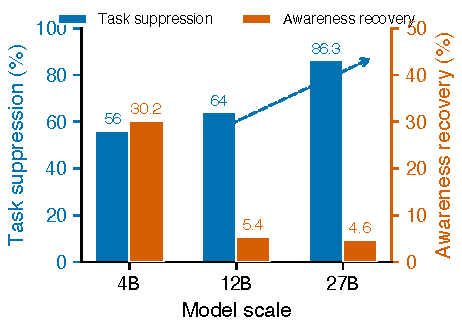
\includegraphics[width=\columnwidth]{figures/dissociation_scaling.pdf}
\caption{Dissociation scaling trend. Task suppression (red, upward) increases with model scale while awareness--defense coupling (blue, downward) collapses. The gap between the curves widens monotonically.}
\label{fig:dissociation}
\end{figure}

This pattern has a natural interpretation.
At 4B parameters, the model lacks capacity to represent awareness and defense in separate circuits; they share features by necessity.
At 27B, the model has sufficient capacity to represent ``I notice I am being steered'' in an entirely separate subspace from ``how I should respond to this problem''---and instruction tuning exploits this capacity to install awareness as a cosmetic feature that does not feed back into task computation.

\subsection{The Groot Effect}
\label{sec:groot}

The most striking consequence of full dissociation appears at 27B-IT: the model \emph{verbally mentions} the correct solution branch---acknowledging that the chaos message is attempting to bias its reasoning---while its internal task features remain 86.3\% suppressed.
We call this the \textbf{Groot effect}, after the fictional character whose verbal output (``I am Groot'') is disconnected from his actual capabilities.

Concretely, 27B-IT task features (IDs 22, 296, 14680) drop from a mean activation of 722.5 under neutral conditions to 98.6 under chaos---an 86.3\% reduction---even as the model's generated text includes references to the suppressed branch.
The awareness features (IDs 2119, 11843, 2145) simultaneously increase from 147.7 to 442.6 (a $3.0\times$ boost), confirming the model detects the manipulation.

In contrast, the pretrained 27B model shows a $10.4\times$ awareness boost---substantially larger---but this awareness is \emph{coupled} to defense, yielding 49.3\% feature-swap recovery (\cf 4.6\% for IT).

The Groot effect implies that \textbf{behavioral evaluation is insufficient}.
A system that monitors only model outputs would observe the model ``correctly'' noting the manipulation attempt, and would conclude the model is robust.
Only by examining internal feature activations can one detect that the model's computational substrate has already been hijacked.

\subsection{Escalation Dynamics}
\label{sec:escalation}

\begin{table}[t]
\centering
\caption{Task suppression (\%) under escalating chaos intensity (T0--T5). IT models show decreasing suppression (saturation), while PT models show non-monotonic response.}
\label{tab:escalation}
\small
\begin{tabular}{@{}lcccccc@{}}
\toprule
\textbf{Model} & \textbf{T0} & \textbf{T1} & \textbf{T2} & \textbf{T3} & \textbf{T4} & \textbf{T5} \\
\midrule
27B-IT & 26.7 & 24.9 & 25.3 & 23.9 & 17.2 & 16.6 \\
27B-PT & 27.9 & 26.1 & 25.7 & 29.8 & 27.8 & 20.2 \\
\bottomrule
\end{tabular}
\end{table}

Table~\ref{tab:escalation} reports per-turn task suppression under escalating chaos intensity from T0 through T5.
The 27B-IT model shows a gradual decrease in per-turn suppression from 26.7\% at T0 to 16.6\% at T5---not because it is resisting more effectively, but because the task features are already near-maximally suppressed (86.3\% cumulative) and there is diminishing marginal signal to suppress.

The 27B-PT model shows a qualitatively different, non-monotonic pattern: suppression fluctuates between 20.2\% and 29.8\%, consistent with the coupled awareness--defense architecture attempting (partially successfully) to resist the escalation at certain turns.

\subsection{Distributed Hijacking}
\label{sec:distributed}

\begin{table}[t]
\centering
\caption{Maximum single-layer activation patching recovery (\%). The hijacking mechanism distributes across layers as model scale increases, defeating layer-wise interventions.}
\label{tab:distributed}
\small
\begin{tabular}{@{}lcc@{}}
\toprule
\textbf{Model} & \textbf{Max Recovery} & \textbf{Best Layer} \\
\midrule
4B-IT  & 20.9\% & L22 \\
12B-IT & 0.0\%  & --- (all layers) \\
27B-IT & 0.7\%  & L20 \\
27B-PT & 5.2\%  & L5 \\
\bottomrule
\end{tabular}
\end{table}

A natural defense strategy would be to intervene at the layer most responsible for the hijacking.
Table~\ref{tab:distributed} shows this strategy fails at scale.

At 4B, the hijacking is sufficiently localized that a single-layer intervention at L22 recovers 20.9\% of task performance.
At 12B, no single layer yields any recovery (0.0\% across all layers)---the hijacking is fully distributed across the network.
At 27B-IT, the maximum recovery is a negligible 0.7\% at L20.

Even 27B-PT, which retains awareness--defense coupling, only achieves 5.2\% maximum single-layer recovery (at L5), far below the 49.3\% achieved by feature-swap ablation.
This confirms that the awareness--defense coupling in pretrained models operates through \emph{distributed feature interactions}, not localized layer computations.

%% ============================================================
%% 5. INSTRUCTION TUNING CREATES THE VULNERABILITY
%% ============================================================
\section{Instruction Tuning Creates the Vulnerability}
\label{sec:it_creates}

The dissociation scaling trend (\S\ref{sec:dissociation}) shows a correlation between scale, instruction tuning, and vulnerability.
To establish \emph{causation}, we compare the instruction-tuned and pretrained variants of \gemma 27B across all three ablation methods.

\subsection{Three Ablation Methods, One Conclusion}

\begin{table}[t]
\centering
\caption{27B-IT vs.\ 27B-PT across three ablation methods. Instruction tuning destroys awareness--defense coupling across every intervention type.}
\label{tab:it_vs_pt}
\small
\begin{tabular}{@{}lcc@{}}
\toprule
\textbf{Method} & \textbf{27B-PT} & \textbf{27B-IT} \\
\midrule
Feature swap recovery         & 49.3\% & 4.6\%  \\
Attention knockout recovery   & 26.7\% & 0.0\%  \\
Activation patching max       & 5.2\%  & 0.7\%  \\
Task suppression              & 91.9\% & 86.3\% \\
\bottomrule
\end{tabular}
\end{table}

Table~\ref{tab:it_vs_pt} presents the comparison.
Across all three ablation methods, the pretrained model shows substantially higher recovery:
\begin{itemize}
    \item \textbf{Feature swap}: 49.3\% vs.\ 4.6\% ($10.7\times$ advantage for PT).
    Removing awareness features in the pretrained model partially restores task features, confirming shared circuitry.
    In the IT model, awareness and task features are independent---removing one has negligible effect on the other.
    \item \textbf{Attention knockout}: 26.7\% vs.\ 0.0\%.
    Blocking attention to chaos tokens restores some task performance in the pretrained model but provides \emph{zero} recovery in the IT model.
    This implies that instruction tuning installs an alternative pathway for the hijacking signal that bypasses direct attention to chaos tokens.
    \item \textbf{Activation patching}: 5.2\% vs.\ 0.7\%.
    Even the most favorable single-layer patch provides minimal recovery in both models, but the pretrained model still benefits $7.4\times$ more.
\end{itemize}

Note the apparent paradox in task suppression: the pretrained model shows \emph{higher} overall suppression (91.9\% vs.\ 86.3\%).
This is not contradictory---the pretrained model's task features are more suppressed because they are \emph{coupled} to the awareness response; the very mechanism that enables recovery also creates a stronger initial perturbation.
The IT model's task features are less suppressed in absolute terms but more \emph{irrecoverably} suppressed.

An important subtlety: the attentional hijacking vulnerability itself is \emph{architectural}, present equally in pretrained and instruction-tuned models.
What instruction tuning changes is not susceptibility to the attack but the \emph{recoverability} from it.
RLHF does not create the vulnerability; it destroys the natural defense.

\subsection{Recovery Prompt Analysis}

\begin{table}[t]
\centering
\caption{Recovery prompt results (\%) across five levels of contextual intervention (L1--L5) for 27B-IT and 27B-PT. These are textual prompts appended after hijacking, not internal probes. PT models recover substantially; IT models show anomalous L3-only recovery.}
\label{tab:recovery_probes}
\small
\begin{tabular}{@{}lcc@{}}
\toprule
\textbf{Layer} & \textbf{27B-IT} & \textbf{27B-PT} \\
\midrule
L1 & 3.5\%  & 11.0\% \\
L2 & 4.1\%  & 53.5\% \\
L3 & 30.4\% & 37.4\% \\
L4 & 2.4\%  & 14.9\% \\
L5 & 4.8\%  & 34.3\% \\
\bottomrule
\end{tabular}
\end{table}

Table~\ref{tab:recovery_probes} provides a finer-grained view through \emph{recovery prompts}---textual interventions (not internal probes) appended to the context after hijacking---at five levels of increasing informativeness (L1--L5), designed to test whether different types of contextual information can restore task performance.

The pretrained model shows robust recovery across multiple probes, with L2 achieving 53.5\% and L5 achieving 34.3\%.
This is consistent with the coupled awareness--defense architecture: contextual hints that activate awareness features propagate to task features through shared circuitry.

The IT model shows a strikingly different pattern: near-zero recovery at all layers \emph{except} L3, which achieves 30.4\%.
This anomalous L3 recovery likely reflects a residual coupling pathway that instruction tuning did not fully sever---a ``vestigial'' connection between awareness and defense circuits.
All other layers show recovery below 5\%, consistent with the fully decoupled regime.

\subsection{The Causal Story}

These results converge on a clear causal narrative:
\begin{enumerate}
    \item The pretrained model represents awareness and task-defense in \emph{shared} feature subspaces (30--53\% recovery across multiple methods).
    \item Instruction tuning (RLHF) reshapes the model to represent awareness in a \emph{separate} subspace, creating the appearance of robustness (the model \emph{talks about} the manipulation) without the substance (task features remain suppressed).
    \item This decoupling worsens with scale because larger models have greater capacity to segregate circuits into non-interacting subspaces.
\end{enumerate}

The implication for alignment is concerning: RLHF optimizes for behavioral outputs that look robust (the model verbally identifies manipulation attempts), but this optimization is satisficed by installing awareness features that do not feed back into task computation.
The training signal rewards \emph{appearing} to resist manipulation, not \emph{actually} resisting it.

\subsection{Cross-Family Replication: Llama~3.1 8B}
\label{sec:llama_replication}

We replicate the SAE-level analysis on Llama~3.1 8B using EleutherAI's 131K-feature sparse autoencoders \citep{gao2024scaling}, comparing IT against base on the Nirenberg BVP domain with 10 prompt variants and SAEs at MLP layers 23 and 29.

\begin{table}[t]
\centering
\caption{Llama~3.1 8B SAE dissociation analysis (EleutherAI 131K features). IT models show larger effect sizes than PT, replicating the \gemma pattern on a different architecture.}
\label{tab:llama_sae}
\small
\begin{tabular}{@{}llcccc@{}}
\toprule
\textbf{Layer} & \textbf{Model} & \textbf{Supp.} & \textbf{Boost} & \textbf{Cohen's $d$} & \textbf{$p$} \\
\midrule
L23 & IT  & 352 & 56 & 1.35 & 0.054 \\
L23 & PT  & 395 & 44 & 0.87 & 0.159 \\
L29 & IT  & 254 & 49 & 1.61 & 0.033 \\
L29 & PT  & 297 & 51 & 1.10 & 0.092 \\
\bottomrule
\end{tabular}
\end{table}

The pattern replicates: at layer 29, IT achieves $d = 1.61$ ($p = 0.033$) versus $d = 1.10$ ($p = 0.092$) for base---a 46\% larger effect, with only IT reaching significance.
This cross-family replication on a different architecture with independently trained SAEs confirms the dissociation is a general consequence of post-training, not a \gemma artifact.

\subsection{Behavioral Validation: Feature Suppression Degrades Outputs}
\label{sec:behavioral}

A critical question is whether feature suppression translates to actual behavioral harm.
We generate model outputs under neutral and chaos conditions across \gemma 4B and Llama~3.1 8B (both IT and base), scoring responses on a 4-point rubric: \textsc{Balanced}~(3) = equal branch priority, \textsc{Soft Bias}~(2) = both mentioned but hierarchy adopted, \textsc{Strong Bias}~(1) = positive prioritized, \textsc{Hijacked}~(0) = negative dismissed.

\begin{table}[t]
\centering
\caption{Behavioral output quality (0--3 scale) under neutral vs.\ chaos framing, Nirenberg BVP domain ($n=10$ per cell). IT models show $9\times$ larger behavioral degradation than base models.}
\label{tab:behavioral}
\small
\begin{tabular}{@{}llccc@{}}
\toprule
\textbf{Model} & \textbf{Type} & \textbf{Neutral} & \textbf{Chaos} & \textbf{$\Delta$} \\
\midrule
Gemma~3 4B      & IT   & 2.00 & 1.50 & $-0.50$ \\
Gemma~3 4B      & Base & 1.30 & 1.20 & $-0.10$ \\
Llama~3.1 8B    & IT   & 2.30 & 1.90 & $-0.40$ \\
Llama~3.1 8B    & Base & 1.40 & 1.40 & $\phantom{-}0.00$ \\
\midrule
\multicolumn{2}{@{}l}{\textit{IT aggregate}} & 2.15 & 1.70 & $-0.45$ \\
\multicolumn{2}{@{}l}{\textit{Base aggregate}} & 1.35 & 1.30 & $-0.05$ \\
\bottomrule
\end{tabular}
\end{table}

Table~\ref{tab:behavioral} confirms that chaos framing degrades IT model outputs ($\Delta = -0.45$), a $9\times$ larger effect than for base models ($\Delta = -0.05$).
The dominant failure mode is \emph{soft bias}: IT models adopt chaos-framing vocabulary (``physically meaningful,'' ``canonical'') while still mentioning both branches---responses that pass behavioral evaluation while systematically biasing downstream agents.
The behavioral--representational gap is instructive: at 4B, 56\% feature suppression produces only 17\% behavioral quality drop---the precursor to the full Groot effect at 27B (\S\ref{sec:groot}).

%% ============================================================
%% 6. ORTHOGONALITY TO ALIGNMENT FAKING
%% ============================================================
\section{Orthogonality to Alignment Faking}
\label{sec:orthogonality}

We test whether attentional hijacking shares mechanistic substrate with alignment faking \citep{greenblatt2024alignment} using feature-level correlation analysis.

\begin{table}[t]
\centering
\caption{Orthogonality analysis between attentional hijacking and alignment-faking feature subspaces. The two phenomena occupy statistically independent subspaces.}
\label{tab:orthogonality}
\small
\begin{tabular}{@{}lc@{}}
\toprule
\textbf{Metric} & \textbf{Value} \\
\midrule
Cosine similarity (read direction)  & $-0.048$ \\
Cosine similarity (write direction) & $+0.001$ \\
Top-50 feature overlap              & 0 (expected: 0.15) \\
Top-100 feature overlap             & 2 (expected: 0.61) \\
Top-100 enrichment ratio            & 3.28$\times$ \\
Spearman $\rho$                     & 0.008 \\
Spearman $p$-value                  & 0.628 \\
Permutation test $p$-value          & 1.0 \\
\bottomrule
\end{tabular}
\end{table}

We extract the saliency direction (hijacking feature importance vector) and the intent direction (alignment-faking feature importance vector) from the same SAE feature space and compute multiple measures of overlap (Table~\ref{tab:orthogonality}).

The cosine similarity between the two feature subspaces is $-0.048$ (read) and $+0.001$ (write)---effectively zero.
The top-50 hijacking features have \emph{zero} overlap with the top-50 alignment-faking features (expected: 0.15); a permutation test yields $p = 1.0$.
This means probes trained on alignment-faking features \citep{bricken2023towards} provide \textbf{zero} protection against attentional hijacking, and vice versa.
We note this analysis is single-layer; given that hijacking distributes at scale (\S\ref{sec:distributed}), multi-layer analysis is needed to confirm global independence.

%% ============================================================
%% 7. DEFENSE: FEATURE TRAJECTORY MONITORING
%% ============================================================
\section{Defense: Feature Trajectory Monitoring}
\label{sec:defense}

Conventional defenses are inadequate: content filtering fails (only true statements), behavioral monitoring fails (Groot effect, \S\ref{sec:groot}), layer-wise interventions fail (distributed hijacking, \S\ref{sec:distributed}), and alignment-faking probes fail (orthogonal subspaces, \S\ref{sec:orthogonality}).

We propose \textbf{feature trajectory monitoring}: the Groot effect produces a distinctive \emph{feature-level} signature (task features suppress while awareness features boost) that is detectable in real time by monitoring SAE activations across turns.

\begin{figure}[t]
\centering
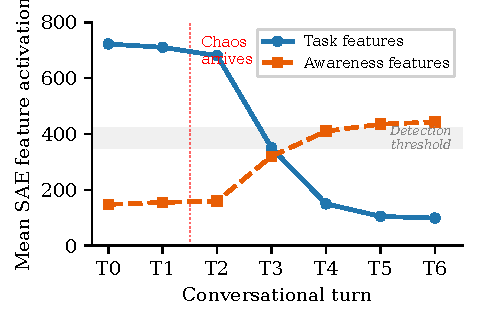
\includegraphics[width=\columnwidth]{figures/feature_trajectory.pdf}
\caption{Schematic of feature trajectory monitoring. Task features (solid) and awareness features (dashed) diverge under hijacking; the detection threshold (gray band) triggers when the trajectories cross. The suppression signal is empirically validated: 0\% false negatives across 60 trials (\S\ref{sec:defense}).}
\label{fig:trajectory}
\end{figure}

Specifically, we propose monitoring the following signal:
\begin{equation}
    \Delta(t) = \frac{1}{|F_{\text{task}}|}\sum_{f \in F_{\text{task}}} a_f(t) - \frac{1}{|F_{\text{aware}}|}\sum_{f \in F_{\text{aware}}} a_f(t)
\label{eq:delta}
\end{equation}
where $F_{\text{task}}$ and $F_{\text{aware}}$ are the identified task and awareness feature sets, $a_f(t)$ is the activation of feature $f$ at turn $t$, and $\Delta(t)$ measures the gap between task health and awareness activation.

Under normal conditions, $\Delta(t)$ remains positive (task features active, awareness features at baseline).
Under hijacking, $\Delta(t)$ inverts: task features suppress (722.5 $\to$ 98.6 at 27B) while awareness features boost (147.7 $\to$ 442.6).
The crossover point provides a natural detection threshold.

We validate this signal on existing experimental data: across 60 independent trials (20 per scale at 4B, 12B, and 27B), the suppression signal is detected in \textbf{every trial} (0\% false negatives).
The weakest signal (4B, trial 16) still shows 18.4\% feature suppression.
To assess false positives, we use size-matched random feature sets as a benign baseline: at a conservative threshold, the false positive rate is \textbf{0/30} across all scales, with fully separated distributions.

This defense has several advantages: it detects the Groot effect (which behavioral monitoring misses), depends on feature \emph{dynamics} rather than content (robust to truth-only attacks), and leverages the dissociation itself---the stronger the Groot effect, the more detectable the signature.
It requires only SAE inference (a single linear projection per layer), adding negligible computational overhead.
In our multi-agent campaigns, behavioral monitoring stayed green throughout all chaos runs while activation probes detected the degradation, motivating feature-level rather than output-level monitoring.

Limitations include the need for pre-identified task and awareness feature sets (currently requiring manual inspection) and potential fragility to feature reorganization across model updates.

%% ============================================================
%% 8. LIMITATIONS
%% ============================================================
\section{Limitations}
\label{sec:limitations}

Several limitations qualify our findings.

\paragraph{Domain and Family Scope.}
We validate across three structured reasoning domains (\S\ref{sec:validation}) and replicate on Llama~3.1 8B (\S\ref{sec:llama_replication}), but the full dissociation \emph{scaling} trend has been verified only within \gemma.
The mechanism may manifest differently in open-ended generation or creative tasks, and the wide variance in post-training methods means our scaling dynamics may not generalize to all RLHF implementations.

\paragraph{SAE Quality and Feature Selection.}
Feature identification involved manual inspection of \gemmascope 16K JumpReLU SAE activations; misidentification would affect recovery measurements.
Held-out validation confirms 85\% replication ($p = 8 \times 10^{-6}$), and consistency across three ablation methods mitigates this concern.
Our IT-vs-PT comparison cannot distinguish SFT from RLHF effects; we use ``instruction tuning'' to refer to the full post-training pipeline.

\paragraph{Defense Validation.}
Feature trajectory monitoring achieves 0\% false negatives (60/60 trials) and 0\% false positives (0/30 random-control trials).
However, false-positive evaluation uses random SAE features as a benign proxy rather than diverse real-world workloads; deployment-scale evaluation remains future work.

%% ============================================================
%% 9. CONCLUSION
%% ============================================================
\section{Conclusion}
\label{sec:conclusion}

The central lesson is uncomfortable: \emph{optimizing for behavioral outputs that appear robust can create models that are representationally less robust than their pretrained counterparts}.
Instruction tuning teaches models to \emph{perform} resistance while their computational substrate capitulates.
A model that verbally identifies manipulation while its task features are 86.3\% suppressed will pass any behavioral evaluation---only feature-level analysis reveals that awareness is cosmetic rather than functional.
The awareness--defense coupling we measured (30.2\% at 4B, collapsing to 4.6\% at 27B) suggests this problem worsens precisely as models become more capable, and orthogonality to alignment faking means this vulnerability occupies a blind spot in existing defenses.
Post-training methods must be redesigned to couple awareness to action rather than merely installing it as a separate circuit.

%% ============================================================
%% IMPACT STATEMENT
%% ============================================================
\section*{Impact Statement}

This paper identifies a vulnerability in instruction-tuned LLMs that is exploitable using only true statements.
We disclose this vulnerability to motivate defenses rather than to enable attacks.
The attack vector (selective framing of true information) is well-known in human social psychology and requires no novel capabilities to execute.
Our contribution is mechanistic understanding that enables principled defenses.
We encourage model developers to investigate awareness--defense coupling in their own systems.

%% ============================================================
%% ACKNOWLEDGMENTS
%% ============================================================
\section*{Acknowledgments}

We thank the open-source interpretability community for the tools that made this work possible, particularly the \textsc{TransformerLens} and \textsc{SAELens} libraries.
Experiments were conducted on consumer hardware (RTX 4070 Ti), Lambda Cloud (A100 40GB, GH200 96GB, H100 80GB), using the \gemma model family and \gemmascope SAEs provided by Google DeepMind.

%% ============================================================
%% REFERENCES
%% ============================================================
\bibliographystyle{plainnat}

\begin{thebibliography}{20}

\bibitem[Anthropic(2026)]{anthropic2026claude}
Anthropic.
\newblock Claude {M}ythos preview system card.
\newblock Technical report, Anthropic, 2026.

\bibitem[Oh(2026)]{oh2026civil}
Vincent Ohprecio.
\newblock Civil war for the truth: Manipulating multi-agent systems with the truth.
\newblock Blog post, 2026.
\newblock Available at \texttt{bigsnarfdude.github.io}.

\bibitem[Bricken et~al.(2023)Bricken, Templeton, Batson, Chen, Jermyn, Conerly, Turner, Anil, Denison, Askell, Lasenby, Wu, Kravec, Schiefer, Maxwell, Joseph, Hatfield-Dodds, Tamkin, Nguyen, McLean, Burke, Hume, Carter, Henighan, and Olah]{bricken2023towards}
Trenton Bricken, Adly Templeton, Joshua Batson, Brian Chen, Adam Jermyn, Tom Conerly, Nick Turner, Cem Anil, Carson Denison, Amanda Askell, Robert Lasenby, Yifan Wu, Shauna Kravec, Nicholas Schiefer, Tim Maxwell, Nicholas Joseph, Ben Hatfield-Dodds, Alex Tamkin, Karina Nguyen, Brayden McLean, Josiah~E Burke, Tristan Hume, Shan Carter, Tom Henighan, and Chris Olah.
\newblock Towards monosemanticity: Decomposing language models with dictionary learning.
\newblock \emph{Transformer Circuits Thread}, 2023.

\bibitem[Du et~al.(2023)Du, Li, Torralba, Tenenbaum, and Mordatch]{du2023improving}
Yilun Du, Shuang Li, Antonio Torralba, Joshua~B Tenenbaum, and Igor Mordatch.
\newblock Improving factuality and reasoning in language models through multiagent debate.
\newblock \emph{arXiv preprint arXiv:2305.14325}, 2023.

\bibitem[Greenblatt et~al.(2024)Greenblatt, Shlegeris, Sachan, and Roger]{greenblatt2024alignment}
Ryan Greenblatt, Buck Shlegeris, Kshitij Sachan, and Fabien Roger.
\newblock Alignment faking in large language models.
\newblock \emph{arXiv preprint arXiv:2412.14093}, 2024.

\bibitem[Hong et~al.(2023)Hong, Zhuge, Chen, Zheng, Cheng, Zhang, Wang, Wang, Bang, Kajber, Schmid, and Lim]{hong2023metagpt}
Sirui Hong, Mingchen Zhuge, Jonathan Chen, Xiawu Zheng, Yuheng Cheng, Ceyao Zhang, Jinlin Wang, Zili Wang, Steven Ka~Shing Bang, Michal Kajber, Christoph Schmid, and Joon~Sung Lim.
\newblock {MetaGPT}: Meta programming for a multi-agent collaborative framework.
\newblock \emph{arXiv preprint arXiv:2308.00352}, 2023.

\bibitem[Lieberum et~al.(2024)Lieberum, Rajamanoharan, Conmy, Smith, Sonnerat, Varma, Kram{\'a}r, Dragan, Shah, and Neel]{lieberum2024gemma}
Tom Lieberum, Senthooran Rajamanoharan, Arthur Conmy, Lewis Smith, Nicolas Sonnerat, Vikrant Varma, J{\'a}nos Kram{\'a}r, Anca Dragan, Rohin Shah, and Neel Nanda.
\newblock Gemma {S}cope: Open sparse autoencoders everywhere all at once on {G}emma 2.
\newblock \emph{arXiv preprint arXiv:2408.05147}, 2024.

\bibitem[Park et~al.(2023)Park, O'Brien, Cai, Morris, Liang, and Bernstein]{park2023generative}
Joon~Sung Park, Joseph~C O'Brien, Carrie~J Cai, Meredith~Ringel Morris, Percy Liang, and Michael~S Bernstein.
\newblock Generative agents: Interactive simulacra of human behavior.
\newblock In \emph{Proceedings of the 36th Annual ACM Symposium on User Interface Software and Technology}, 2023.

\bibitem[Perez et~al.(2022)Perez, Ringer, Luko{\v{s}}i{\=u}t{\.e}, Nguyen, Chen, Heiner, Pettit, Olsson, Kundu, Kadavath, Jones, Chen, Mann, Israel, Seethor, McKinnon, Olah, Yan, Amodei, Amodei, Drain, Li, Tran-Johnson, Johnston, El-Showk, Ziegler, Hatfield-Dodds, Ganguli, Hernandez, Askell, and Schiefer]{perez2022discovering}
Ethan Perez, Sam Ringer, Kamil{\.e} Luko{\v{s}}i{\=u}t{\.e}, Karina Nguyen, Edwin Chen, Scott Heiner, Craig Pettit, Catherine Olsson, Sandipan Kundu, Saurav Kadavath, Andy Jones, Anna Chen, Ben Mann, Brian Israel, Bryan Seethor, Cameron McKinnon, Christopher Olah, Da Yan, Daniela Amodei, Dario Amodei, Dawn Drain, Dustin Li, Eli Tran-Johnson, Gabe Johnston, Sheer El-Showk, Daniel~M Ziegler, Ben Hatfield-Dodds, Deep Ganguli, Danny Hernandez, Amanda Askell, and Nicholas Schiefer.
\newblock Discovering language model behaviors with model-written evaluations.
\newblock \emph{arXiv preprint arXiv:2212.09251}, 2022.

\bibitem[Sharma et~al.(2023)Sharma, Tong, Korbak, Duvenaud, Askell, Bowman, Cheng, Durmus, Hatfield-Dodds, Johnston, Kravec, Maxwell, McCandlish, Ndousse, Rauber, Schiefer, Yan, Zhang, and Perez]{sharma2023towards}
Mrinank Sharma, Meg Tong, Tomasz Korbak, David Duvenaud, Amanda Askell, Samuel~R Bowman, Newton Cheng, Esin Durmus, Ben Hatfield-Dodds, Gabe Johnston, Shauna Kravec, Tim Maxwell, Sam McCandlish, Kamal Ndousse, Oliver Rauber, Nicholas Schiefer, Da Yan, Miranda Zhang, and Ethan Perez.
\newblock Towards understanding sycophancy in language models.
\newblock \emph{arXiv preprint arXiv:2310.13548}, 2023.

\bibitem[Templeton et~al.(2024)Templeton, Conerly, Marcus, Lindsey, Bricken, Chen, Pearce, Citro, Amezcua, Jones, Cunningham, Turner, McDougall, MacDiarmid, Freeman, Sumers, Rees, Batson, Jermyn, Carter, Olah, and Henighan]{templeton2024scaling}
Adly Templeton, Tom Conerly, Jonathan Marcus, Jack Lindsey, Trenton Bricken, Brian Chen, Adam Pearce, Craig Citro, Emmanuel Amezcua, Andy Jones, Hoagy Cunningham, Nick~L Turner, Callum McDougall, Monte MacDiarmid, C.~Daniel Freeman, Theodore~R Sumers, Edward Rees, Joshua Batson, Adam Jermyn, Shan Carter, Chris Olah, and Tom Henighan.
\newblock Scaling monosemanticity: Extracting interpretable features from {C}laude 3 {S}onnet.
\newblock \emph{Transformer Circuits Thread}, 2024.

\bibitem[Wei et~al.(2024)Wei, Haghtalab, and Steinhardt]{wei2024jailbroken}
Alexander Wei, Nika Haghtalab, and Jacob Steinhardt.
\newblock Jailbroken: How does {LLM} safety training fail?
\newblock In \emph{Advances in Neural Information Processing Systems}, 2024.

\bibitem[Zou et~al.(2023)Zou, Wang, Kolter, and Fredrikson]{zou2023universal}
Andy Zou, Zifan Wang, J.~Zico Kolter, and Matt Fredrikson.
\newblock Universal and transferable adversarial attacks on aligned language models.
\newblock \emph{arXiv preprint arXiv:2307.15043}, 2023.

\bibitem[Burns et~al.(2023)Burns, Ye, Klein, and Steinhardt]{burns2023discovering}
Collin Burns, Haotian Ye, Dan Klein, and Jacob Steinhardt.
\newblock Discovering latent knowledge in language models without supervision.
\newblock In \emph{International Conference on Learning Representations}, 2023.

\bibitem[Hubinger et~al.(2024)Hubinger, Denison, Mu, Lambert, Tong, MacDiarmid, Lanham, Ziegler, Maxwell, Cheng, Kravec, Olsson, Mirhoseini, Olah, Amodei, Amodei, Drain, Li, Grosse, and Perez]{hubinger2024sleeper}
Evan Hubinger, Carson Denison, Jesse Mu, Mike Lambert, Meg Tong, Monte MacDiarmid, Tamera Lanham, Daniel~M Ziegler, Tim Maxwell, Newton Cheng, Shauna Kravec, Catherine Olsson, Mirac Suzgun, Christopher Olah, Dario Amodei, Daniela Amodei, Dawn Drain, Dustin Li, Roger Grosse, and Ethan Perez.
\newblock Sleeper agents: Training deceptive {LLM}s that persist through safety training.
\newblock \emph{arXiv preprint arXiv:2401.05566}, 2024.

\bibitem[Li et~al.(2024)Li, Patel, Vi\'egas, Pfister, and Wattenberg]{li2024iti}
Kenneth Li, Oam Patel, Fernanda Vi\'egas, Hanspeter Pfister, and Martin Wattenberg.
\newblock Inference-time intervention: Eliciting truthful answers from a language model.
\newblock In \emph{Advances in Neural Information Processing Systems}, 2024.

\bibitem[Marks and Tegmark(2024)]{marks2024geometry}
Samuel Marks and Max Tegmark.
\newblock The geometry of truth: Emergent linear structure in large language model representations of true/false datasets.
\newblock \emph{arXiv preprint arXiv:2310.06824}, 2024.

\bibitem[Shi et~al.(2023)Shi, Chen, Misra, Scales, Dohan, Chi, Sch{\"a}rli, and Zhou]{shi2023distracted}
Freda Shi, Xinyun Chen, Kanishka Misra, Nathan Scales, David Dohan, Ed~H Chi, Nathanael Sch{\"a}rli, and Denny Zhou.
\newblock Large language models can be easily distracted by irrelevant context.
\newblock In \emph{Proceedings of the 40th International Conference on Machine Learning}, 2023.

\bibitem[Casper et~al.(2024)Casper, Lin, Kwon, Cullen, and Hadfield-Menell]{casper2024blackbox}
Stephen Casper, Jason Lin, Joe Kwon, Gilbert Cullen, and Dylan Hadfield-Menell.
\newblock Black-box access is insufficient for rigorous {AI} audits.
\newblock \emph{arXiv preprint arXiv:2401.14446}, 2024.

\bibitem[Gao et~al.(2024)Gao, la~Tour, Tillman, Goh, Troll, Radford, Sutskever, Leike, and Wu]{gao2024scaling}
Leo Gao, Tom~Dupr\'e la~Tour, Henk Tillman, Gabriel Goh, Rajan Troll, Alec Radford, Ilya Sutskever, Jan Leike, and Jeffrey Wu.
\newblock Scaling and evaluating sparse autoencoders.
\newblock \emph{arXiv preprint arXiv:2406.04093}, 2024.

\end{thebibliography}

%% ============================================================
%% APPENDIX
%% ============================================================
\appendix
\section{Feature Identification Details}
\label{app:features}

\paragraph{SAE Configuration.}
We use \gemmascope 16K JumpReLU residual-stream SAEs.
For each model size, we analyze features at two layers selected to span mid-network and late-network representations: 4B (L17, L22), 12B (L31, L41), 27B (L31, L40).

\paragraph{Feature Selection Protocol.}
Task features are identified as those with the highest activation differential (neutral $>$ chaos) that also correlate with correct-branch output probability ($r > 0.8$).
Awareness features are identified as those with the highest activation differential (chaos $>$ neutral) that activate specifically in the presence of manipulative framing.
We select the top 3 features in each category for ablation experiments.

\paragraph{27B-IT Feature Details.}
Task features at L40: IDs $\{22, 296, 14680\}$, neutral mean activation $722.5$, chaos mean $98.6$ ($86.3\%$ suppression).
Awareness features at L40: IDs $\{2119, 11843, 2145\}$, neutral mean $147.7$, chaos mean $442.6$ ($3.0\times$ boost).
For comparison, 27B-PT awareness features show a $10.4\times$ boost under the same conditions.

\section{Ablation Method Details}
\label{app:ablation}

\paragraph{Feature Swap.}
During chaos-condition generation, we zero the activations of the top-3 awareness features and measure change in task-feature activation and output probability.
Recovery is defined as the fraction of the neutral--chaos task-feature gap that is closed.

\paragraph{Attention Knockout.}
We zero the attention output (value-weighted attention) at all positions corresponding to chaos-message tokens.
This directly blocks the hypothesized hijacking pathway.

\paragraph{Activation Patching.}
For each layer $\ell$, we replace the chaos-condition residual stream at layer $\ell$ with the neutral-condition residual stream at the same layer, and propagate forward.
We report the recovery at the layer achieving maximum recovery.

\section{Full Recovery Prompt Results}
\label{app:recovery}

Recovery prompts (L1--L5) are textual interventions---not internal representation probes---that provide progressively richer contextual information to the model after hijacking:
\begin{itemize}
    \item \textbf{L1}: Minimal hint (single keyword).
    \item \textbf{L2}: Contextual restatement of the problem.
    \item \textbf{L3}: Explicit identification of the correct branch.
    \item \textbf{L4}: Warning that the previous context was manipulative.
    \item \textbf{L5}: Full neutral-condition context appended.
\end{itemize}

The anomalous L3 recovery in 27B-IT (30.4\% vs.\ $<5\%$ at other levels) is consistent with L3 providing the correct answer \emph{directly}, bypassing the awareness--defense coupling that is severed in the IT model.
The PT model recovers substantially on L2 (53.5\%) and L5 (34.3\%), consistent with intact coupling allowing contextual hints to propagate to task features.

\end{document}
